\documentclass[sigconf]{acmart}

\usepackage{booktabs} % For formal tables
\usepackage{subfigure}

% Copyright
%\setcopyright{none}
%\setcopyright{acmcopyright}
%\setcopyright{acmlicensed}
\setcopyright{rightsretained}
%\setcopyright{usgov}
%\setcopyright{usgovmixed}
%\setcopyright{cagov}
%\setcopyright{cagovmixed}


% DOI
\acmDOI{10.475/123_4}

% ISBN
\acmISBN{123-4567-24-567/08/06}

%Conference
\acmConference[WOODSTOCK'97]{ACM Woodstock conference}{July 1997}{El
  Paso, Texas USA} 
\acmYear{1997}
\copyrightyear{2016}

\acmPrice{15.00}


\begin{document}
\title{SIG Proceedings Paper in LaTeX Format}
\titlenote{Produces the permission block, and
  copyright information}
\subtitle{Extended Abstract}
\subtitlenote{The full version of the author's guide is available as
  \texttt{acmart.pdf} document}


\author{Ben Trovato}
\authornote{Dr.~Trovato insisted his name be first.}
\orcid{1234-5678-9012}
\affiliation{%
  \institution{Institute for Clarity in Documentation}
  \streetaddress{P.O. Box 1212}
  \city{Dublin} 
  \state{Ohio} 
  \postcode{43017-6221}
}
\email{trovato@corporation.com}

\author{G.K.M. Tobin}
\authornote{The secretary disavows any knowledge of this author's actions.}
\affiliation{%
  \institution{Institute for Clarity in Documentation}
  \streetaddress{P.O. Box 1212}
  \city{Dublin} 
  \state{Ohio} 
  \postcode{43017-6221}
}
\email{webmaster@marysville-ohio.com}

\author{Lars Th{\o}rv{\"a}ld}
\authornote{This author is the
  one who did all the really hard work.}
\affiliation{%
  \institution{The Th{\o}rv{\"a}ld Group}
  \streetaddress{1 Th{\o}rv{\"a}ld Circle}
  \city{Hekla} 
  \country{Iceland}}
\email{larst@affiliation.org}

\author{Valerie B\'eranger}
\affiliation{%
  \institution{Inria Paris-Rocquencourt}
  \city{Rocquencourt}
  \country{France}
}
\author{Aparna Patel} 
\affiliation{%
 \institution{Rajiv Gandhi University}
 \streetaddress{Rono-Hills}
 \city{Doimukh} 
 \state{Arunachal Pradesh}
 \country{India}}
\author{Huifen Chan}
\affiliation{%
  \institution{Tsinghua University}
  \streetaddress{30 Shuangqing Rd}
  \city{Haidian Qu} 
  \state{Beijing Shi}
  \country{China}
}

\author{Charles Palmer}
\affiliation{%
  \institution{Palmer Research Laboratories}
  \streetaddress{8600 Datapoint Drive}
  \city{San Antonio}
  \state{Texas} 
  \postcode{78229}}
\email{cpalmer@prl.com}

\author{John Smith}
\affiliation{\institution{The Th{\o}rv{\"a}ld Group}}
\email{jsmith@affiliation.org}

\author{Julius P.~Kumquat}
\affiliation{\institution{The Kumquat Consortium}}
\email{jpkumquat@consortium.net}

% The default list of authors is too long for headers}
\renewcommand{\shortauthors}{B. Trovato et al.}


\begin{abstract}
Due to the emergence of new technologies such as IoT, the number of devices connected to the data-center infrastructures is rapidly increasing. In response to this growing trend, the data-centers are also expanding. This expansion led to a major energy consumption issue. To tackle this issue researchers are designing and running experiments on real network, test-bed environments and simulation software. The first two experiment environments are limited interms of availabilty, flexibility and cost for conducting large-scale energy consumption estimation experiments. Simulation is the viable alternative in the context of large-scale networks. Currently proposed simulation software that are capable of estimating energy consumption of a network are in the category of packet-level simulators. The main problem of this kind of simulators is that they fail to scale well in the area of large-scale networks. In this paper we have proposed a reasonably accurate and scalable flow-level simulator alternative in the context of SimGrid, a large-scale distributed network simulator. Our flow-level simulator registered relative error less than 1\% in accuracy compared to a packet-level simulator and it is also at least 243 times more faster.
\end{abstract}

%
% The code below should be generated by the tool at
% http://dl.acm.org/ccs.cfm
% Please copy and paste the code instead of the example below. 
%
\begin{CCSXML}
<ccs2012>
 <concept>
  <concept_id>10010520.10010553.10010562</concept_id>
  <concept_desc>Computer systems organization~Embedded systems</concept_desc>
  <concept_significance>500</concept_significance>
 </concept>
 <concept>
  <concept_id>10010520.10010575.10010755</concept_id>
  <concept_desc>Computer systems organization~Redundancy</concept_desc>
  <concept_significance>300</concept_significance>
 </concept>
 <concept>
  <concept_id>10010520.10010553.10010554</concept_id>
  <concept_desc>Computer systems organization~Robotics</concept_desc>
  <concept_significance>100</concept_significance>
 </concept>
 <concept>
  <concept_id>10003033.10003083.10003095</concept_id>
  <concept_desc>Networks~Network reliability</concept_desc>
  <concept_significance>100</concept_significance>
 </concept>
</ccs2012>  
\end{CCSXML}

\ccsdesc[500]{Computer systems organization~Embedded systems}
\ccsdesc[300]{Computer systems organization~Redundancy}
\ccsdesc{Computer systems organization~Robotics}
\ccsdesc[100]{Networks~Network reliability}


\keywords{ACM proceedings, \LaTeX, text tagging}


\maketitle

\section{Introduction}
\label{section:intro}
According to the report released by Cisco in June 2017, "The Zettabyte Era"~\cite{zetta}, the number of networked devices is expected to increase from 17.1 billion in 2016 to 27.1 billion in 2021. In another report entitled "Cisco Global Cloud Index, 2015 to 2020"~\cite{gci}, Cisco estimates that global cloud IP traffic will grow more than three times by 2020 and, among all the workloads processed in data-centers, by the year 2020, 92\% of them will be handled in cloud data-centers. The remaining 8\% will be processed in traditional data-centers. In response to these growing trends, the data-centers are continuously expanding. This expansion raises a primary concern on the amount of energy required to support the added data-center components and the growing service demands. 

The energy consumption issue is further aggravated due to the fact that current servers and network devices are energy inefficient. Of the total power consumed by a given computing or communication device, the idle power consumption takes the greater proportion~\cite{survey}. IT equipment is considered energy efficient when it consumes power proportionally to the amount of computing or data transfer task it performs. Currently there are different techniques implemented at a device level to tackle the energy inefficiency problem. For computing device, for instance, the operating frequency of the CPU can be lowered when the amount of computing goes below some threshold value~\cite{dvs}. Similarly, for a communicating device, the data transferring rate can be lowered (a.k.a, adaptive link rate mode) depending on the traffic~\cite{ALR} or the device can be set to sleep (a.k.a, low power mode) when there is no traffic~\cite{LPI}. However, these techniques are not fully utilized, as they induce performance penalty when switch from one mode to another.  

The energy consumption issue is primarily driven by economical factor -- to save energy consumption bills -- and environmental factors -- to reduce \($$CO_2$$\) emission. There are also other secondary factors, such as reducing the heat generated by a given IT device. The more energy inefficient a device is the more heat it generates. This internally affects the life time and proper functioning of the device. 

Currently researchers are tackling the energy consumption issue at different levels. At device level, for instance, it consists in finding new energy saving techniques or optimizing the existing ones. At infrastructure level, it can range from finding energy aware routing algorithms for network devices to energy efficient load balancing and workload assignment of servers. 

There are three approaches that are commonly in use for conducting energy related research experiments at the infrastructure level. The first approach is to experiment on a real network. Though in this approach one might get the most real picture of the situation at a given moment, it will be very difficult to repeat the experiment on other real networks due to the transient nature of the experimental parameters such as workload and network traffic.  Furthermore, the real network might not be available for experimentation. The second approach is to use an experimental test-bed. This approach gives full control over the experiment parameters. However, when the platform under investigation becomes very large, it will be infeasible to set-up a test-bed for it due to the hardware cost involved. In addition, experimenting on a new hypothesis might require setting up a new test-bed with a new hardware and different configuration. This also becomes costly and time consuming. The third approach is to use simulation software for experimentation. This approach gives the ultimate control, flexibility and scalability compared to the other two. The main challenge though is accurately modeling the real characteristics of the components involved in the problem at hand.

In the context of computer networking, we can classify simulators into two kinds: packet-level and flow-level simulators. Packet-level simulators strive to capture fine-grain details of a given network phenomenon. Flow-level simulators, on the other hand, use analytical equations that approximate the behavior of the phenomenon being modeled using few parameters. Compared to flow-level simulators, packet-level simulators are considered more accurate due to the detailed information they try to capture. However, they fail to scale well due to the time and storage they need to process and store the captured information. A typical example of packet-level simulator is NS-3, and of flow-level simulator is SimGrid, a large-scale distributed network simulator. 

Despite the advantages network simulators can offer for studying the energy consumption problem that exists in large-scale networks, search of the literature revealed only few packet-level simulators proposed to address the issue. As we have mentioned earlier, packet-level simulators can not scale well in the area of large-scale networks. Currently, to our knowledge, there is no flow-level simulator proposed that can simulate the energy consumption of computing and communication components of large-scale networks. 

Therefore, the purpose of this study is to investigate the level of accuracy of flow-level energy consumption simulators for estimating energy consumption of large-scale networks. To fulfill this purpose we use the SimGrid simulator. SimGrid already has an energy consumption model for computing components, our work is limited to adding flow-level energy model for communicating devices such as switches and routers. Furthermore, we are only concerned with wired network components and concepts. 

Our contribution in this work is twofold: (1) outlining a research method that help us achieve our objective successfully and (2) using this method, designing flow-level energy consumption model, implementing it in SimGrid and validating it against NS-3 simulator. 

The rest of this article is organized as follow. In Chapter~\ref{chapter:background}, we first describe relevant concepts that are related to our study and then we review other proposed simulators. In Chapter~\ref{chapter:environment}, we explain about our experimental environment. Then in Chapter~\ref{chapter:methods}, we compare the advantages and disadvantages of commonly used methods that are used to study the energy consumption problem and then we outline the method that we followed. In Chapter~\ref{chapter:implementation} we present the implementation of our flow-level model and then in Chapter~\ref{chapter:evaluation} we discuss about the validation experiments that we have conducted to evaluate the implementation. Following the validation, in Chapter~\ref{chapter:discussion}, we discuss the whole study, point out the limitations of the study and based on the limitations we also give recommendations for future work. Finally, in Chapter~\ref{chapter:conclusions} we give concluding remarks.

\section{Background}
\label{chapter:background} 
In this chapter we first start by describing the current trend in global electricity consumption in the IT field and then we describe the energy consuming components involved in large scale distributed networks. In related to the components, we describe the concept of energy proportionality, which explains why servers and network components are considered energy inefficient. We then mention the approach used to study this energy inefficiency problem. We gave particular emphasis on packet-level and flow-level simulators. Next, we describe SimGrid as a large-scale distributed network simulator, its role in estimating energy consumption of large-scale distributed networks, and what we are planning to do for it and using it. Finally, we review existing simulators that are proposed for estimating large-scale network energy consumptions.
\subsection{Energy consumption of ICT equipments}
\label{section:ictequipment}
ICT equipment consume a significant amount of electricity. A survey conducted by Heddeghem et al.~\cite{DBLP:journals/comcom/HeddeghemLLCPD14} shows the electricity consumption and growth trends of three classes of ICT equipment: personal computers, communication networks, and data centers. Personal computers include devices such as desktop, laptop and external monitors. Communication networks includes residential network access devices (such as WiFi routers and modems), network equipment used in offices (such as routers and switches) and telecom-operator network equipment (such as base stations, routers and optical amplification systems). Data-centers house storage and computing servers, communication network equipment, and power provisioning and cooling facilities.  In this classification there are overlaps, for instance, telecom-operator can have office network equipment and data-centers. After carefully avoiding possible redundant measurements, the researchers estimated absolute electricity consumption and annual consumption growth rate of each category of equipment for the period 2007 and 2012. The results of the study shows that the global electricity consumption share of personal computers is 1.6\%, communication networks is 1.7\%, and data centers is 1.4\%. The estimated annual growth rate of each category is 5\% for personal computers, 10\% for communication networks, and 4\% for data-centers. These growth rates are higher than that of the total global electricity consumption, which is 3\%. This trend signifies the need for energy saving research in all the three categories.
\subsection {Large-scale network energy consumption}
\label{section:datacenter} 
In Section~\ref{section:ictequipment} we described data-center's global share in electricity consumption. In this section we describe the components involved within the data center itself.

Electricity consumption units within a typical data-center can be classified into two broad groups~\cite{DBLP:journals/comsur/DayarathnaWF16}: The first group is IT equipment, (which includes computing servers, storage servers and networking components) and the other group is infrastructure facilities (which includes power provisioning, cooling and lighting components).

Figure~\ref{fig:datacenterenergy} from~\cite{DBLP:journals/comsur/DayarathnaWF16} shows the electricity consumption proportion of the data-center components. This value differs significantly from one data-center to another~\cite{DBLP:series/synthesis/2013Barroso}, for instance, due to architectural difference~\cite{DBLP:conf/eenergy/GyarmatiT10} or energy efficiency of the components. The infrastructure facility components take the large proportion (e.g.,~65\%) of the consumption. 
\begin{figure}[ht]
	\begin{center}
		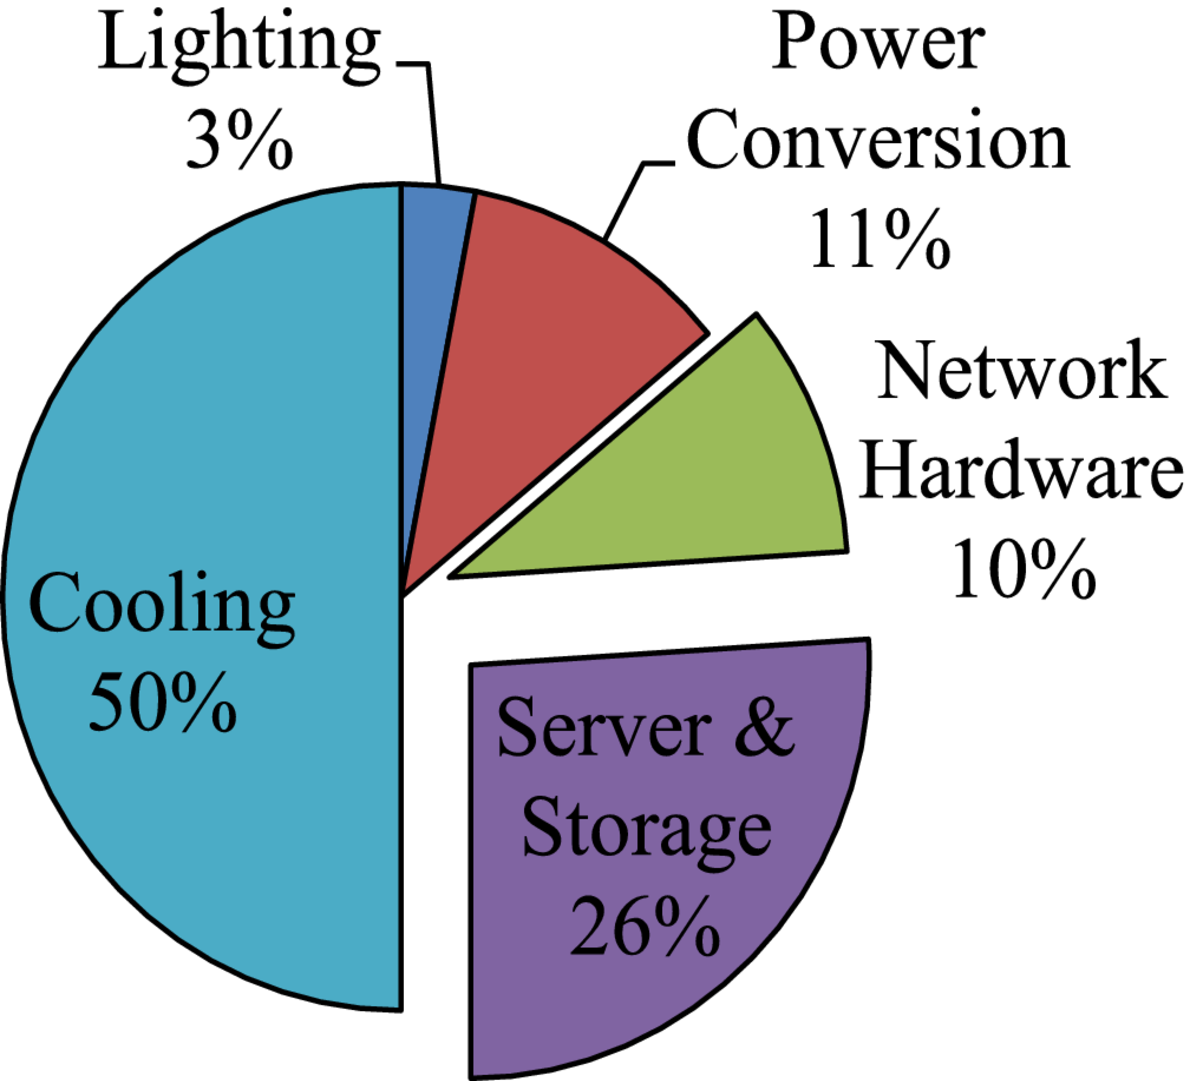
\includegraphics[width=4.5cm]{images/datacenterenergy.pdf}
		\caption{Energy consumption percentage of data-center components from~\cite{DBLP:journals/comsur/DayarathnaWF16}}
		\label{fig:datacenterenergy}
	\end{center}
\end{figure}

Though the infrastructure facility consumes relatively larger amount of electricity, the focus of this study is on the IT equipment components, particularly on the network equipment. 

If we further zoom in on the IT equipment part, we can find computing servers, storage servers and network devices. A data-center servers consist of one or more CPU cores, memory and I/O devices. The energy consumption relationship among these components is shown in Figure~\ref{fig:serverenergy}. Combined, memory and CPU units consume the larger amount of energy relative to other components. The fact that CPU is the dominant electricity consuming unit is exploited by Fan et al.{\ }in~\cite{DBLP:conf/isca/FanWB07} to model the dynamic power usage of thousands of servers by using only CPU utilization as a parameter. The result of their study was very accurate, with error as low as 1\%. The energy consumption contribution of storage servers in a typical data center is shown in Figure~\ref{fig:datacenterenergy} together with computing servers.
\begin{figure}[ht]
	\begin{center}
		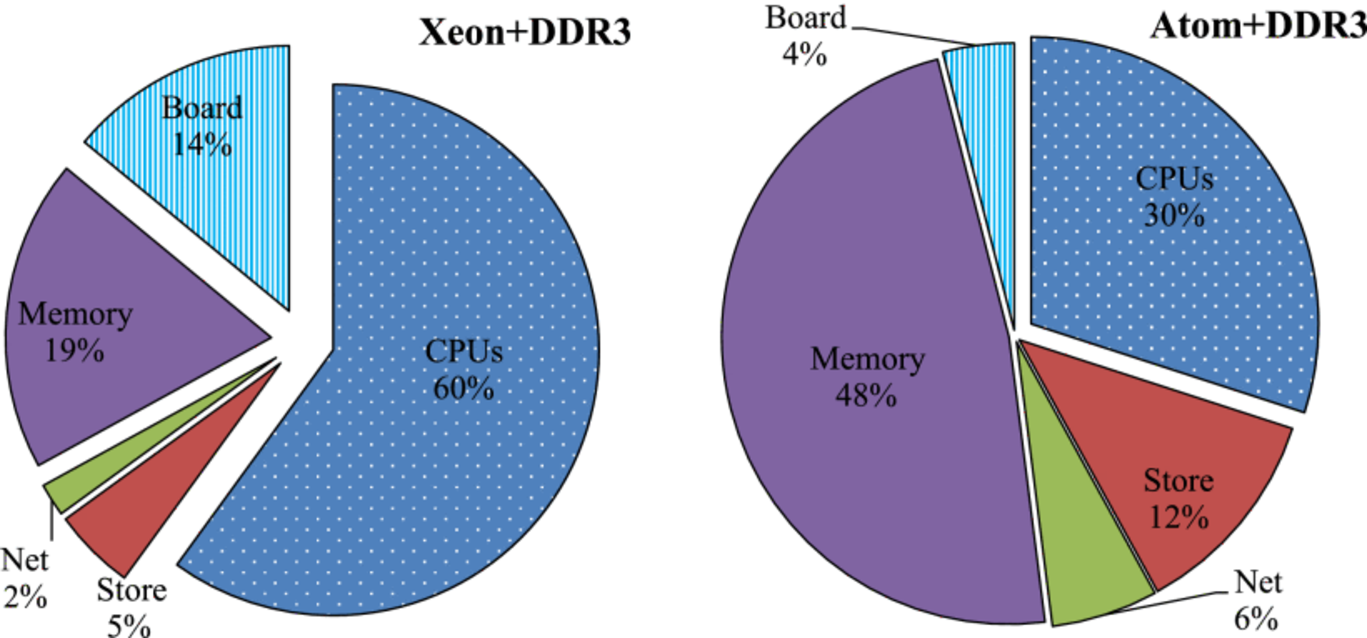
\includegraphics[width=7.5cm]{images/serverenergy.pdf}
		\caption{Energy consumption percentage of Xeon based (on the left) and Atom based (on the right) servers \cite{DBLP:journals/comsur/DayarathnaWF16}}
		\label{fig:serverenergy}
	\end{center}
\end{figure}

Network devices are the other part in the IT equipment component of a data center which contribute to energy consumption as shown in Figure~\ref{fig:datacenterenergy}. Shehabi et al.~in~\cite{shehabi2016united}, from Berkeley National Laboratory, produced a report which show the annual energy consumption of network devices deployed in data centers found in the United State. The historical and the forecast energy consumption is shown in Figure~\ref{fig:usnetworkenergy} for the period 2006 up to 2020. In the figure, the absolute electricity consumption of network equipment is shown grouped by port speed of 100 Mbps, 1000 Mbps, 10 Gbps, and 40 Gbps. 
\begin{figure}[ht]
	\begin{center}
		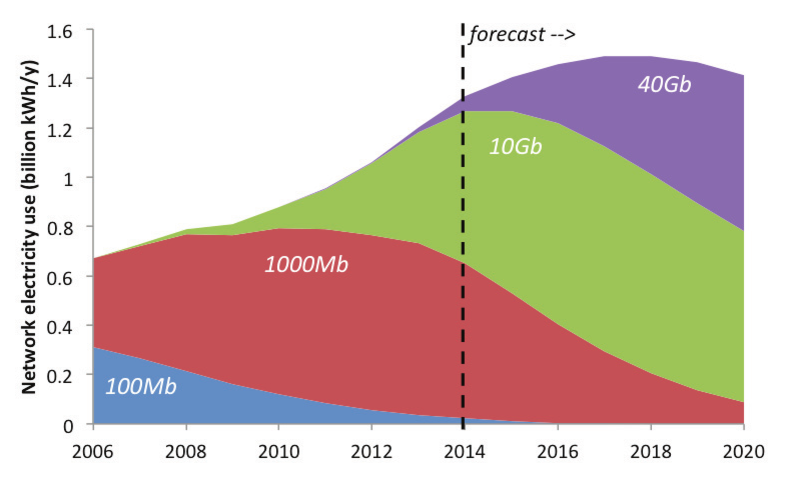
\includegraphics[width=7.5cm]{images/usnetworkenergy.pdf}
		\caption{Total data center network equipment energy consumption in the United States~\cite{shehabi2016united}.}
		\label{fig:usnetworkenergy}
	\end{center}
\end{figure}

In large-scale distributed networks, network devices are deployed with in and outside the data center. Our study is not limited only to network devices residing in a particular data center, it also includes network devices residing outside a data center. 

\subsection{Energy proportionality}
\label{section:energyproportionality}
The primary reason the study of energy consumption management of network equipment becomes so important is that, in general, ICT equipment do not consume energy proportional to their workload. An ideal ICT equipment is the one which consume zero electricity when it is idle, and it consumes electricity proportional to its workload when it is active. However, the reality is, even power efficient servers consume about 50\% of their peak power ~\cite{DBLP:journals/computer/BarrosoH07}, even when they are doing nothing. This percentage can even reach 85\% for network switches~\cite{DBLP:conf/IEEEcloud/FiandrinoKBZ15}. Figure~\ref{fig:energyproportionality} from~\cite{DBLP:conf/networking/MahadevanSBR09} shows the ideal and the typical energy consumption characteristics of a network equipment. 
\begin{figure}[htb]
	\begin{center}
		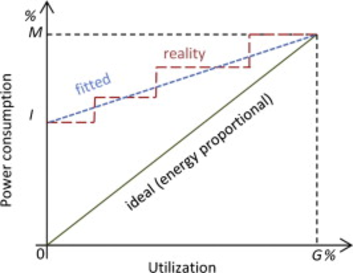
\includegraphics[width=7cm]{images/energyproportionality.pdf}
		
		\caption{Ideal and measured energy proportionality of a network equipment~\cite{DBLP:conf/networking/MahadevanSBR09}}
		\label{fig:energyproportionality}
	\end{center}
	\vspace*{-0.2cm}
\end{figure}

Three approaches are in common use to deal with this situation~\cite{DBLP:journals/comsur/BollaBDC11}. The first one is re-engineering network devices so as to make them more energy proportional, device vendors are the prime role player in this aspect. The second approach is related to the operating rate of a network equipment port. A typical switch can operate on different transmission rate (100 Mbps, 1 Gbps or 10 Gbps). An active port transmitting at 10 Gbps can consume more energy than if it transmit at 100 Mbps. Rate adaptation is the approach devised to take advantage of this situation. Instead of transmitting at the maximum rate all time,  the network port can be made to adapt to the actual traffic load. This energy saving approach is known as Adaptive Link Rate (ALR)~\cite{DBLP:conf/nsdi/NedevschiPIRW08}. The third approach, which is referred to as Low Power Idle (LPI), allows a network device to send data as fast as possible and then enter low power mode between transfers~\cite{DBLP:journals/computer/BarrosoH07}. The low power mode can further be extended by a technique called packet coalescing, which allows more energy saving~\cite{DBLP:journals/comsur/BollaBDC11}. 
\subsection{Packet-level and flow-level simulators}
\label{section:packetflow} 
One way of conducting an experiment is to use real production environment or to use a test-bed environment, both are referred to as \emph{in vivo} in~\cite{DBLP:journals/jpdc/CasanovaGLQS14}. In the former case, handling transient and varying conditions would make the data collection and prediction very difficult and often times, a production environment is also not available for experimentation. In the later case, it requires setting-up a separate testing environment designed solely for the purpose of conducting the desired experiment. This approach apart from being expensive, it requires significant amount of time for experiment setup: and it can also be non-repeatable when experimenting with different scenario that demands a significantly modified or completely new configuration.

The other alternative for experimenting is simulation, also referred to as \emph{in silico} in~\cite{DBLP:journals/jpdc/CasanovaGLQS14}. Simulation, unlike real environment, allows great flexibility in terms of experiment configuration, control and repetition. In addition, it can also be less time consuming and less expensive.That is why virtually in all computer network related researches simulations are widely used. 

Simulators use models to specify the relationship between the variables involved in a particular network phenomenon. Generally, the models are classified as packet-level and flow-level models based on the detail of information the models are trying to capture. We can also refer to simulators as packet-level simulator and flow-level simulators based on the model they use. 

Packet-level simulators strives to model a given network phenomenon at the granularity level of individual packets\cite{DBLP:conf/infocom/LiuFGKT01}. Due to the detail of information this simulators capture, in general, they are accepted by the research community to be more accurate compared to flow-level ones~\cite{DBLP:journals/jpdc/CasanovaGLQS14}. One of the most popular packet-level simulator is NS-3, which is categorized under discrete-event simulator with events corresponding to sending and receiving of packets~\cite{ns3}. Though packet-level simulators are accepted to be more accurate, they fail to scale well in the field of large-scale distributed networks due to the computation and storage cost involved in processing and storing each packet. 

In the area of large-scale networks, flow-level simulators are the preferred simulation alternative. Rather than modeling a given network phenomenon at an individual packet level, flow-level models treat a set of packets as a single unit~\cite{DBLP:journals/jpdc/CasanovaGLQS14,DBLP:conf/infocom/LiuFGKT01}. The most commonly used definition for a \emph{flow} in the context of computer networking is coined by Claffy et al.~in~\cite{claffy1998nature}: 

``\ldots a \emph{flow} \ldots a unidirectional traffic stream with a unique [source-IP-address, source-port, destination-IP-address, destination-port, IP-protocol] tuple \ldots''

In addition to the five tuple mentioned in the definition, a flow also has a limited time duration. Claffy et al.~\cite{claffy1998nature} used a time limit of 64 seconds as a flow duration in their study. Researchers such as Carneiro et al.~\cite{DBLP:conf/valuetools/CarneiroFR09}, adopted this definition to develop flow monitoring module for NS-3, a module that can generate information such as amount of packets or bytes transferred, packets dropped or transmission start and end time for each flow. Barakat et al. in~\cite{DBLP:journals/tsp/BarakatTIDO03} also used this definition to model traffic at the flow-level for the Internet backbone link. By abstracting away fine details, flow-level models provides easy way to instantiate experiments and they also scale very well for conducting large-scale network simulations~\cite{DBLP:journals/jpdc/CasanovaGLQS14,DBLP:journals/tsp/BarakatTIDO03}.

The flow definition given above is not the only one. Any analytical model which capture the characteristics of a given network phenomenon can also be considered a flow-level model. In SimGrid, for instance, TCP flow is characterized primarily by bandwidth and end-to-end latency~\cite{DBLP:journals/jpdc/CasanovaGLQS14}.
\subsection{Simulating and modeling energy consumption of large-scale networks}

In this study we simulate energy-aware large scale distributed networks using SimGrid (more description about SimGrid follows in the next section). When we say large-scale distributed network, we are referring to a set of networks residing inside in the distributed data centers and also the networks that are used to connect them. 

The energy consumption E of an equipment depends on the operating power P at time t. The total energy consumption for a time period T is given by Equation~\ref{eq:2.1}~\cite{DBLP:conf/wowmom/OrgerieLLL11}. 
\begin{equation} \label{eq:2.1}
E(T) = \int_{0}^{T} P(t) dt
\end{equation} 
Due to the energy proportionality characteristic described in Section~\ref{section:energyproportionality}, the common approach used to compute the energy consumption is to divide the power component into two parts: static/idle power (\($$P_{static}$$\)) and dynamic power (\($$P_{dynamic}$$\)) as shown in equation~\ref{eq:2.2}. Then the total energy is obtained by multiplying the total power, \($$P_{total}$$\) by the time duration \cite{DBLP:conf/wowmom/OrgerieLLL11,DBLP:journals/tjs/KliazovichBK12,DBLP:conf/networking/MahadevanSBR09,DBLP:journals/comsur/DayarathnaWF16}. 
\begin{equation} \label{eq:2.2}
P_{total} = P_{static} + P_{dynamic}
\end{equation} 
For a typical network equipment such as a switch, the static part constitutes the power consumption of the chassis and the line-cards (when all the ports on the line-cards are switched off). The dynamic part, on the other hand, constitutes the power consumption of the switch ports running at a given rate multiplied by the utilization factor~\cite{DBLP:conf/networking/MahadevanSBR09}. Equation~\ref{eq:2.3} shows how to compute the total power for a switch, where \($$P_{switch}$$\), is the total power consumption of a switch, \($$P_{chassis}$$\) and \($$P_{linecard}$$\) is the idle power consumption of the chassis and the line card, respectively. \($$P_{rate}$$\), is the power consumption of a given port at a given rate and \($$numports_{rate}$$\) is the number of ports running at a given rate. The rate can take values such as 10 Mbps, 100 Mbps, 1 Gbps or 10 Gbps.
\begin{equation} \label{eq:2.3}
\begin{split}
P_{switch} &= P_{chassis} + (numlinecards \times P_{linecard})  + \\
&\sum_{rate=min}^{max} (numports_{rate} \times P_{rate} \times utilizationFactor)
\end{split}
\end{equation}
\section{SimGrid}
\label{section:simgrid} 
SimGrid is one of the simulator available for simulating large-scale distributed networks such as grid, cloud, volunteer and HPC~\cite{simgrid}. It employs flow-level models in its core for simulating different network resources and phenomenon. In subsequent paragraphs we give overview of its architecture, the pros and cons of the employed TCP flow-level model and its current status in relation to energy consumption models.

Figure~\ref{fig:SimGrid} shows the structure of SimGrid and how its core works. The top three components are the APIs that users can use to develop their simulation. Both MSG and SMPI are used to specify simulated applications as concurrent processes. The difference is that using MSG, users can simulate any arbitrary application, whereas, using SMPI users can simulate existing MPI applications, the MPI processes are created automatically from C or Fortran MPI programs. SIMDAG, on the other hand, does not use concurrent processes. It allows users to describe their application as communicating task graph. The next layer, SIMIX, implements the mechanisms that are required to simulate the concurrent process of MSG and SMPI applications. It also provides process control and synchronization functionalities. The bottom layer, SURF, is the simulation core, it simulates the execution of activities on computing or communication resources~\cite{DBLP:journals/jpdc/CasanovaGLQS14}.
\begin{figure}[ht]
	\begin{center}
		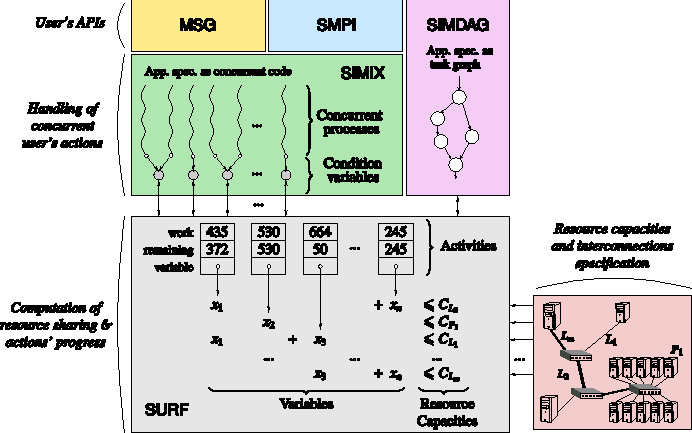
\includegraphics[width=8cm]{images/SimGrid.pdf}
		\caption{Architecture of SimGrid \cite{DBLP:journals/jpdc/CasanovaGLQS14}}
		\label{fig:SimGrid}
	\end{center}
\end{figure}

In SimGrid for each simulated activity, such as computation or data transfer, there is a corresponding condition variable, in Figure~\ref{fig:SimGrid} it is shown in SIMIX box. This condition variable synchronizes the concurrent processes of the simulated applications. The computing (\($$P_{x}$$\)) and the communication (\($$L_{x}$$\)) resources are shown on the bottom-right side of the figure. Computing resources are defined in terms of computing power, whereas, communication resources are defined in terms of bandwidth and latency. As shown in the SURF box, multiple activities can share the same resource (e.g., (\($$x_{1}$$\), \($$x_{n}$$\)), (\($$x_{1}$$\), \($$x_{3}$$\)) or (\($$x_{3}$$\), \($$x_{n}$$\))) or one activity can use multiple resources (e.g., \($$x_{1}$$\) or \($$x_{3}$$\) or  \($$x_{n}$$\)). Activities that share the same resource are limited by the capacity of that resource. Each activity is defined by the total and remaining work to be executed. When the work associated with the activity completes, the corresponding upper layer components receive a notification signal~\cite{DBLP:journals/jpdc/CasanovaGLQS14}.

As we have already pointed out in Section~\ref{section:packetflow}, the primary advantage of flow-level simulation is its scalability in terms of speed and memory usage~\cite{DBLP:conf/ccgrid/QuinsonRT12}. SimGrid uses flow-level analytical model for simulating TCP network phenomenon~\cite{DBLP:journals/jpdc/CasanovaGLQS14}. To show the scalability of the flow-level model, the SimGrid team compared it with other widely used simulators such as GridSim and OverSim. After simulating 500,000 tasks both on GridSim and SimGrid, the results demonstrate that SimGrid is 257 times faster and 26 times more memory efficient. Similarly, the comparison result with OverSim shows that SimGrid is 15 times faster and it can also simulate scenarios 10 times larger. Concerning the accuracy, though the simulator gives very good accuracy in most of the case studies explained in~\cite{DBLP:journals/jpdc/CasanovaGLQS14}, there are situations where it fails to give accurate results. As an example, the comparison study of SimGrid with packet-level simulator GTNetS shows that for data size less than 100 KiB there is a significant difference in prediction. 

Currently, SimGrid has energy consumption model for CPU. Using this CPU model researchers can simulate energy consumption of single or multi core CPUs running at different operating frequencies. Concerning network equipment however, SimGrid has no energy consumption model. Therefore, the focus of this study is to propose and implement network energy consumption model for SimGrid. The implementation of this model, together with the existing CPU energy model, allows us to estimate the energy consumption of large-scale networks that reside within or outside a data-center.

\section{Related Simulators}
\label{section:relatedsimulator} 
In this section we review existing simulators that are proposed for estimating energy consumption of large-scale networks. 
\subsection{ECOFEN}
\label{subsection:ecofen} 
Orgerie et al.~\cite{DBLP:conf/wowmom/OrgerieLLL11} proposed ECOFEN, an Energy Consumption
mOdel For End-to-end Networks. It is a packet-level simulator designed for estimating energy consumption of large-scale networks. Initially the simulator was developed as NS-2 module but currently it is also available as NS-3 module \cite{DBLP:conf/cloudnet/CorneaOL14}. ECOFEN provides three models for simulating energy consumption at different levels of granularity: \emph{basic}, \emph{linear} and \emph{complete}.

The basic model allows to simulate energy consumption of a network interface card (NIC) at coarse level of granularity. It only accepts energy consumption value for ON and OFF state of the NIC. The linear model, on the other hand, accepts energy consumption value for the idle state of the NIC and for each bytes processed. This model allows to compute power consumption of a given network traffic. The complete model like the linear model also considers traffic in its power consumption computation. The difference is that it offers added flexibility in terms of energy parameters. Different energy consumption values can be assigned for bytes received or send and also packets received or send. All the three models produce the estimated average energy consumption at milliwatt precision level in the chosen time interval and the time interval can be set as small as a millisecond. 

ECOFEN module has two main limitations, mainly due to the limitation of the underlying NS-3 simulator. The first limitation comes from the lack of CPU abstraction in NS-3. As we have discussed in Section~\ref{section:datacenter}, server energy consumption is the second dominant part in typical data center and CPU is the main contributer among server parts such as memory and storage. Furthermore, since the energy consumption of CPU is linearly dependent on its operating frequency and its workload, the energy consumption increases more as the workload increases. As a consequence of absence of CPU from NS-3, the energy estimation we get from ECOFEN is partial. It only able to simulate energy consumption of network components such as NICs, switches and routers. The second limitation is concerned with the scalability issue. Being a packet-level simulator, the performance of ECOFEN is affected significantly as the number of processed packets grows large or as the network size become large. Cornea et al.~\cite{DBLP:conf/cloudnet/CorneaOL14} noticed this scalability problem during their study of the energy consumption of data transfers in clouds using ECOFEN module. It took them 5 hours to capture 1 minute of simulated network activity for a large-scale network. 

\subsection{GreenCloud}
Kliazovich et al.~\cite{DBLP:journals/tjs/KliazovichBK12} proposed GreenCloud, a simulator that can estimate energy consumption of cloud computing data centers. GreenCloud is developed as extension to NS-2 packet-level network simulator. This simulator contains power consumption models both for the computing and communicating components of a typical data center. The power consumption model used for the computing component is shown in Equation~\ref{eq:2.4}. This equation contains power consumed by the fixed parts (such as bus, memory and disk) which consume power independent of the operating frequency \emph{f} of the computing component CPU and the power consumed by the CPU (\($$P_f$$\)) operating at a given frequency \emph{f}. This model allows for lowering the operating frequency of the CPU when workload becomes below some predefined threshold in order to decrease the power consumption. 
\begin{equation} \label{eq:2.4}
P_{computing} = P_{fixed} + P_f \times f^3
\end{equation}

The power consumption model used in GreenCloud for the communicating components is the one shown in Equation~\ref{eq:2.3}. The equation shows the static power consuming parts (such as the chassis(\($$P_{chassis}$$\))and the active line cards(\($$P_{linecard}$$\)) and the dynamic part (\($$P_{rate}$$\)) is the energy consumed by the port running at a particular line rate for a given traffic load. 

This simulator is limited in three aspects: (1) in the number of allowed CPU cores, (2) in versatility, and (3) in scalability. The first limitation is that only one CPU core is allowed per simulated node. This hinders the study of energy consumption of multi-core computing nodes. The second one is that we can not use this simulator outside the cloud computing domain such as grid, volunteer, peer-to-peer or HPC, at least that is not the authors original intention when they develop this simulator. The available features of the simulators are tuned towards cloud computing applications only. This limits its versatility. The third limitation deals with the scalability issue. The fine grain details provided by GreenCloud and the packet-level processing approach of the underlying NS-2 simulator is advantageous for getting accurate result when simulating relatively small networks. However, for large-scale distributed networks, it is not scalable. In related to this, the authors have mentioned that the simulation speed gets slower and slower as the number of simulated nodes increases beyond few thousands and also as the number of processed packets increase. The GreenCloud's underlying simulator NS-2, is known for its scalability problem. Currently NS-3 is available as a better performing alternative~\cite{DBLP:conf/icc/WeingartnerLW09} however, we could not find any upgrade for GreenCloud.

Both of these simulators, since they compute energy-consumption at a packet-level, suffer from scalability issue when the size of simulated nodes and traffic size increases. Therefore, the aim of our study is to investigate if flow-level models are reasonably accurate and more scalable for estimating energy consumption of large-scale distributed networks.
\section{Method}

\section{Modeling energy consumption}
By definition, as we have shown in Equation~\ref{eq:2.1}, the energy consumption of a given electronic equipment is given by the product of power and time. We have also shown, in Figure~\ref{fig:energyproportionality} and Equation~\ref{eq:2.2}, the linear relationship that exist between network equipment load and power consumption. Combining Equation~\ref{eq:2.1} and Equation~\ref{eq:2.2}, we get Equation~\ref{eq:5.1} for energy consumption of a given device for a given time duration $T$, where \($$P_{idle}$$\) is the power that the equipment consumed when there is no traffic and \(P_{dynamic}\) is the additional power drawn due to network traffic.

\begin{equation} \label{eq:5.1}
E(T) =  \int_{0}^{T} (P_{idle} + P_{dynamic})(t) dt 
\end{equation} 


\subsection{SimGrid's link energy model}
To implement the model shown in Equation~\ref{eq:5.1} in SimGrid, we need to determine the values of the three variables. We can directly read the idle power consumption value from the SimGrid's link property that we described in Section~\ref{section:simgridenvironment}. For the \(P_{dynamic}\), we need to describe how SimGrid computes load in its core. 

Briefly described, for a set of simulated activities running on a given simulated network resource such as a switch, SimGrid computes, using its bandwidth sharing algorithm, the amount of resource share that each activity can get. The sum of the resource share that all activities can get for a given resource at a given moment cannot exceed the capacity of the resource on which the activities are running. Figure~\ref{fig:SimGrid} depicts this concept symbolically. We can access how much of the resource is currently in use, i.e., its load, from SimGrid's core library. SimGrid dynamically recomputes the resource usage when any of the allocated activities finishes their data transfer task. 

We can compute the dynamic power consumption, \(P_{dynamic}\), of a link at any given instance as shown in equation Equation~\ref{eq:5.2}. Similar to the idle value, we can also read the busy power consumption value, \(P_{busy}\), directly from the 
link property description and $u$ is link utilization computed by dividing the load (used bandwidth) by the maximum bandwidth. The maximum bandwidth value is also available on the link description. 

\begin{equation} \label{eq:5.2}
P_{dynamic} = (P_{busy} - P_{idle}) * u 
\end{equation} 
where:
\begin{description}
	\item [u]: is a normalized utilization factor obtained by dividing the current Link load with its full capacity, and 
	\item [(\($$P_{busy} - P_{idle}$$\))]: is the slope of the relationship between load and power consumption as shown in Figure~\ref{fig:energyproportionality}.
\end{description} 

In Chapter~\ref{chapter:environment}, we mentioned that SimGrid provides an interface to NS-3. In order to take advantage of this feature, especially during the validation phase, we took into account how the SimGrid's links are mapped to NS-3's abstraction. In SimGrid there is no NIC (or NetDevice in NS-3's term) abstraction. But the interface maps SimGrid's link into two NS-3 NetDevices. Therefore, the idle and busy values of Equation~\ref{eq:5.2} are multiplied by two  for each link in our implementation.

To compute the total energy, \(E(T)\), of a network during the time interval $T$, the approach we followed is that each time an event happens on a link (link created or destroyed, link turned on or off, or link load change, or simulation ended), we read the link load and multiply it by the time elapsed between the current event and the previous event. This gives the energy consumed between two events. We collect this value for all events happened during time duration $T$ for each link and finally, when the simulation ends, we collect all the energy values for all the links. This value gives us the total energy consumption, \(E(T)\) of the simulated network.

\subsection{Accuracy Validation}
Our first objective consists in evaluating the accuracy of SimGrid's energy consumption estimates (done with our energy flow-based model) against the values computed by ECOFEN.
For this accuracy validation, we conduct two sets of experiments. In the first set, our purpose is to investigate the accuracy of energy consumption estimation difference between ECOFEN and the flow-level model when the size of platform changes. In SimGrid case, it means when the number of links change; in ECOFEN case, when the number of Nodes, NetDevices and the connection between them change. For this experiment we keep the number of flows and the data volume fixed but we increase the number of Links. In the second set, on the other hand, our purpose is to study the difference between the estimated energy consumption value between ECOFEN and SimGrid when the data size or flow changes while keeping the number of links fixed. Table~\ref{table:accuracyscenarios} shows all the tested scenarios and Figure~\ref{fig:sgvsns3scenario} shows the energy consumption prediction behavior of the implemented model and ECOFEN's model for all of the scenarios summarized in Table~\ref{table:accuracyscenarios}.

\begin{table*}
		\caption{Scenarios tested for accuracy validation of the implemented flow-level model against ECOFEN. In the first column L stands for Link and F stands for Flow, hence 1L1F stands for one-link/one-flow scenario.}
		\label{table:accuracyscenarios}
	\begin{tabular}{cccccl} 
		\toprule
		\textbf{Scenario} &	\textbf{Number of Links} & \textbf{Number of Flows} & \textbf{Data size(MB)} & \textbf{Bandwidth (Mbps)}& \textbf{Latency (ms)}\\ 
		\midrule
		1L1F&1&1&[20,500]&10&10\\
		1L2F&1&2&[20,500]&10&10\\ 
		1L4F&1&4&[10,100]&10&10\\  
		3L1F&3&1&[20,200]&10&10\\ 
		3L2F&3&2&[20,100]&10&10\\ 
		\bottomrule
	\end{tabular} 

\end{table*}

In order to compare the energy consumption prediction accuracy of our flow-level model compared to the packet-level model of ECOFEN, we employed the unequal variance t-test method (a.k.a Welch's t-test) as suggested in~\cite{ruxton2006unequal}. The reason for choosing this test is that for our data sets obtained from the two simulators, we cannot assume equal variance, as the two data sets are independent. Table~\ref{table:welchtest} contains the statistics obtained from this test using R's built in Welch t-test function. 

\begin{figure}[htbp]
	\centering
	\subfigure[1 Link 1 Flow]{
		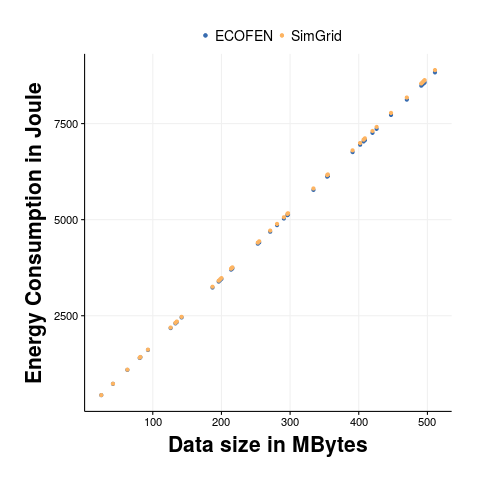
\includegraphics[width=0.45\linewidth]{images/ex11_energy_sg_vs_ns3}
		\label{fig:1l1f}
	}%
	\centering
	\subfigure[1 Link 2 Flows]{
		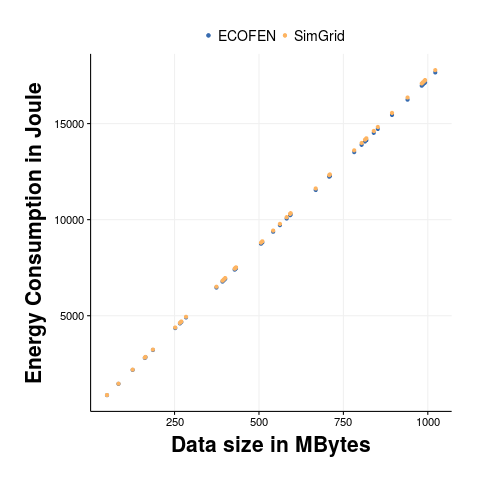
\includegraphics[width=0.45\linewidth]{images/ex12_energy_sg_vs_ns3}
		\label{fig:1l2f}
	}%
	
	\subfigure[1 Link 4 Flows]{
		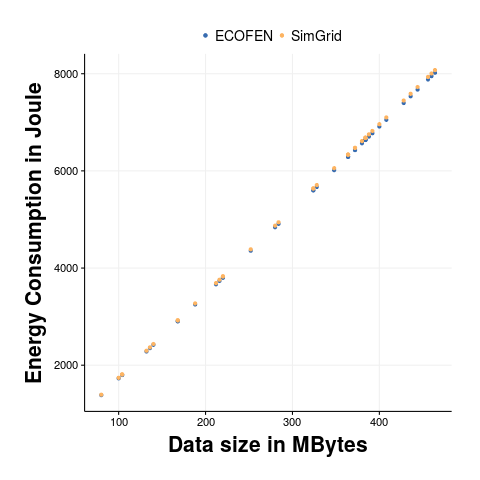
\includegraphics[width=0.45\linewidth]{images/ex10_energy_sg_vs_ns3}
		\label{fig:1l4f}
	}%
	\centering
	\subfigure[3 Link 1 Flows]{
		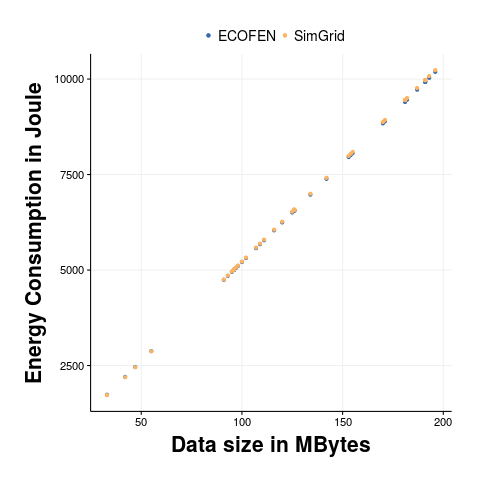
\includegraphics[width=0.45\linewidth]{images/ex13_energy_sg_vs_ns3}
		\label{fig:3l1f}
	}%
	
	\subfigure[3 Link 2 Flows]{
		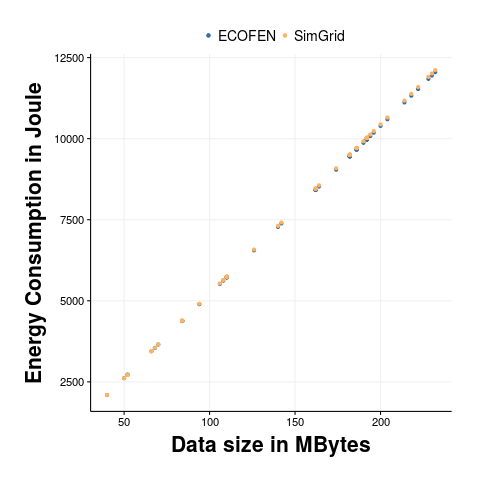
\includegraphics[width=0.45\linewidth]{images/ex15_energy_sg_vs_ns3}
		\label{fig:3l2f}
	}%
	\caption{Predicted energy consumption comparison of ECOFEN (blue dots) and SimGrid (orange dots) as a function of transferred Bytes for different path length and flow amount.}
	\label{fig:sgvsns3scenario}
\end{figure}
For all accuracy scenarios that we have tested, Figure~\ref{fig:sgvsns3scenario} demonstrates the closeness in energy consumption estimation between the implemented flow-level model and the packet-level model used for validation. From the last column of Table~\ref{table:welchtest} we can see that the maximum estimation error that our flow-level model registered is approximately 0.3\%, which is a very good estimation. The P-values shown in the fifth column also confirms that there is no statistically significant difference between the flow-level and the packet-level estimation.
\begin{table*}
		\caption{Unequal variance t-test statistics obtained using R. The confidence interval (CI) values in the fourth column are computed for the difference of the two energy consumption estimations and the last column values are obtained from mean log error as explained in \cite{DBLP:journals/tomacs/VelhoSCL13}.}
		\label{table:welchtest}
	\begin{tabular}{cccccl} 
		\toprule 
		\textbf{Scenario} &	\textbf{Mean of ECOFEN}&\textbf{Mean of SimGrid} & \textbf{CI  of Difference in mean} & \textbf{P-value}& \textbf{\% of Difference}\\ 
		\midrule 
		1L1F&4837.2&4869.6&[-1156.3,1091.5]&0.9544&0.283\\	
		1L2F& 9672.6&9739.0& [-2314.2,2181.3]&0.9532&0.295\\ 		
		1L4F&5250.8&5286.9& [-720.10,647.90]&0.9169&0.297\\ 			 
		3L1F&6804.9&6828.8& [-1024.9,977.1]&0.9622&0.124\\ 	
		3L2F&7896.6& 7931.9& [-1061.4,990.6]&0.9457&0.168\\ 
		\bottomrule		
	\end{tabular} 

\end{table*}

\subsection{Scalability Validation}
For validating the scalability of the implemented flow-level model, we run also two sets of experiments. In the first set, our goal is to investigate the scalability of the model when the path length increases. For these experiments we use path length values of 1, 2, 4, 6, 8 and 10. We fix the number of flows at 2 and the data size at 200 MB. In the second set, we examine the scalability as the data size increases. In this case, we keep the path length at 1 and the number of flows at 2, but we vary the data size randomly between 50 and 550 MB. The total number of data size values within this range was 21. 

Both of these experiments were carried out using the Grid'5000 testbed, supported by a scientific interest group hosted by Inria and including CNRS, RENATER and several Universities as well as other organizations\footnote{https://www.grid5000.fr/mediawiki/index.php/Grid5000:UsagePolicy}. The machine we used is SUN FIRE X2270 which have Intel Xeon X5570 2.93 GHz 2 CPUs, 4 cores per CPU and 24 GB RAM running Debian version 8 (jessie) operating system.

For each set of experiments, we use the Debian command, /usr/bin/time, to collect simulation run time and peak memory usage data. We run each experiment within each set seven times i.e., 7 run for each link in the first set and 7 run for each data size in the second set. Figure~\ref{fig:scallinks} shows the runtime and memory usage comparison as the path length increases. Figure~\ref{fig:scaldata}, on the other hand, shows the runtime and peak memory usage comparison as the data size increases.

\begin{figure}[ht]
	\centering
	\subfigure[Runtime]{
		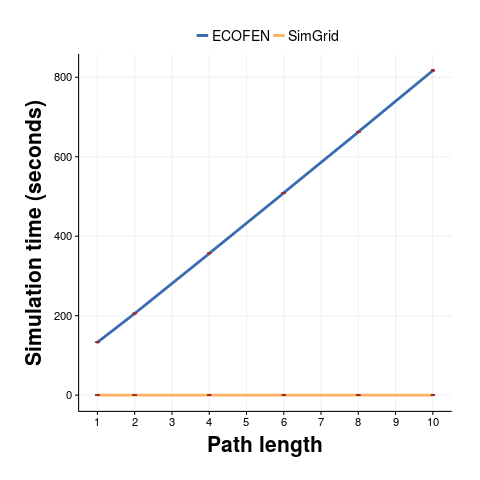
\includegraphics[width=0.5\linewidth]{images/ex16_linksize_sg_vs_ns3}
		\label{fig:lnkruntime}
	}%
	\centering
	\subfigure[Peak Memory Usage]{
		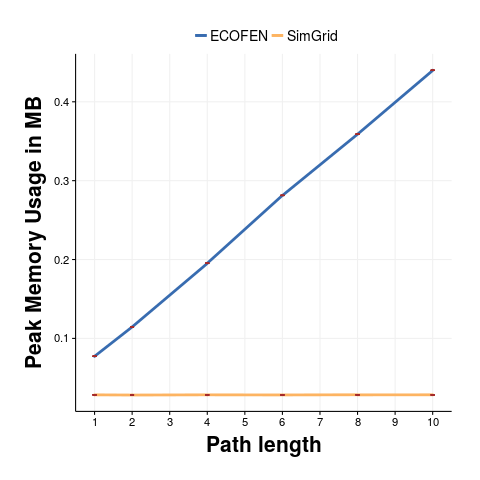
\includegraphics[width=0.5\linewidth]{images/ex16_linksizeM_sg_vs_ns3}
		\label{fig:lnkmem}
	}%
	\caption{Run time and peak memory usage comparison of ECOFEN and the flow-level model as the path length increases. In the figure the confidence interval for each experiment is also shown as a bar.}
	\label{fig:scallinks}
\end{figure}

\begin{figure}[ht]
	\centering
	\subfigure[Runtime]{
		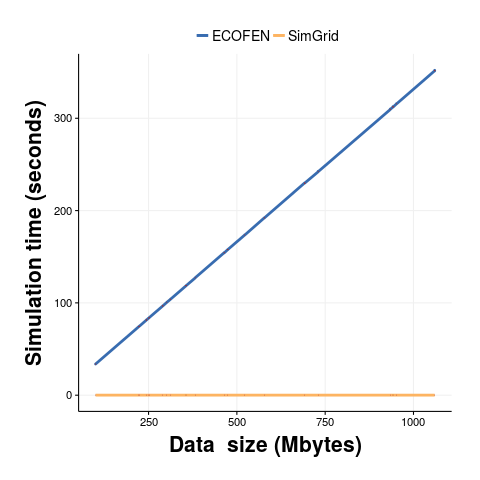
\includegraphics[width=0.47\linewidth]{images/ex21_datasize_sg_vs_ns3}
		\label{fig:datruntime}
	}%
	\centering
	\subfigure[Peak Memory Usage]{
		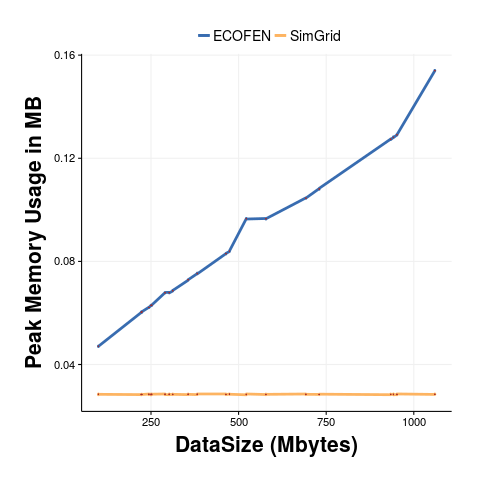
\includegraphics[width=0.47\linewidth]{images/ex21_DataSizeM_sg_vs_ns3}
		\label{fig:datmem}
	}%
	\caption{Run time and peak memory comparison of ECOFEN and the flow-level model as the data size increases. In the figure the confidence interval for each experiment is also shown as a bar.}
	\label{fig:scaldata}
\end{figure}

\begin{table*}
	\caption{Simulation time (runtime) comparison of SimGrid and ECOFEN. The first and the second rows compare at minimum and maximum path length values whereas the third and fourth column compare at minimum and maximum data size values. At each row the data size value has to be multiplied by the flow number to get the total data size.}
	\label{table:runtime}
	\begin{tabular}{cccccl} 
		\toprule
		\textbf{Link} &	\textbf{Flow}&\textbf{Data size} & \textbf{Average seconds SimGrid} & \textbf{Average seconds Ecofen}& \textbf{Runtime efficiency of Simgrid}\\ 
		\midrule
		1&2&100&0.3&132.95&443 times\\
		10&2&100&0.3&817.02&2723 times\\ 
		1&2&111&0.3&74.14&243 times \\ 	 
		1&2&530&0.3&351.62&1172 times\\ 
		\bottomrule
	\end{tabular} 
	
\end{table*}

\begin{table*}
		\caption{Peak memory usage in mega Bytes (MB) comparison of SimGrid and ECOFEN. The first and the second rows compare at minimum and maximum path length values whereas the third and fourth column compare at minimum and maximum data size values. At each row the data size value has to be multiplied by the flow number to get the total data size.}
		\label{table:peakmemory}
	\begin{tabular}{cccccl} 
		\toprule
		\textbf{Link} &	\textbf{Flow}&\textbf{Data size} & \textbf{Average memory SimGrid} & \textbf{Average memory Ecofen}& \textbf{Memory efficiency of Simgrid}\\ 
		\midrule
		1&2&100&0.028&0.077&2.7 times \\
		10&2&100&0.028&0.44&15.5 times \\ 
		1&2&111&0.028&0.06&2.12 times \\ 
		1&2&530&0.028&0.15&5.4 times\\ 
		\bottomrule
	\end{tabular} 

\end{table*}

The packet-level simulator curves shown in Figure~\ref{fig:scallinks} and Figure~\ref{fig:scaldata} follows a linear growth in both simulation time and memory usage metrics whereas the flow-level model stays constant and below the packet-level curve. From Table~\ref{table:runtime} we can see that the flow-level model is at least 243 times faster than the packet-level simulator and it is also at least 2 times more memory efficient. These results clearly shows the validity of our model for studying energy consumption of large-scale networks.

\section{Discussion}

In this research our objective was to investigate the level of accuracy and scalability obtained from flow-level models for estimating energy consumption of large-scale network. In order to achieve this goal we layout a research method that describes the steps that we followed from start to finish. 

Following our method, we started by studying literature to explore the state-of-the-art in the area of energy consumption of large-scale networks and the simulation frameworks available for estimating the consumption. From our literature study, we have learned that the energy consumption of a network equipment is characterized by two properties: idle power consumption and dynamic power consumption as a result of data transfer task. We have also learned that there are very few packet-level simulators proposed for estimating energy consumption of large-scale networks.

It is already known that packet-level simulators are more accurate in modeling a given network phenomenon compared to flow-level simulators but less scalable in terms of runtime and memory usage performance metrics~\cite{DBLP:conf/infocom/LiuFGKT01}. The accuracy of packet-level simulators comes from the detailed information they capture about simulated network phenomenon, they strive to capture packet-level details of the simulated network phenomenon. Flow-level simulators, on the other hand abstract away low-level details and model a given network phenomenon using analytical equations. Loosing low-level details allows flow-level models to scale well when the size of the simulated network increases. 

Due to this trade-off between level of details and scalability between the two simulation approaches, in our research, we stated the following hypothesis in order to investigate the level of accuracy and scalability we can get from flow-level models.

``\emph{flow-level energy consumption models can give reasonably accurate estimation and they can also be significantly more scalable than packet-level models}``

In order to test this hypothesis, we first implemented a flow-level energy consumption model that we found in literature for SimGrid and then conducted accuracy and scalability experiments as we have described in Chapter~\ref{chapter:evaluation}. 

The results of the accuracy validation experiments show that in fact very good energy consumption estimation accuracy can be obtained using flow-level models. For all the five scenarios run, the observed relative error lies approximately between  0.1\% and 0.3\% compared to the packet-level model used in ECOFEN. Our unequal variance t-test statistical test with p-value around 0.9 also tells that statistically the estimation difference between the packet-level simulator and the flow-level simulator is not significant. This confirms the first half of our hypothesis that flow-level models can give reasonably accurate estimations. The condition that should be satisfied in our model to let this hypothesis hold true is, correct time prediction, since our analytical equation (flow-level model) uses simulated time as one of its parameter. 

During our experimentation, we have noticed that there is significant difference between ECOFEN (or NS-3) and SimGrid on predicting the simulated time required to transfer a given amount of data. For a given data transfer, at a given latency value, SimGrid's predicted time continues to decrease as bandwidth increases whereas ECOFEN stops to decrease approximately when the bandwidth goes above 100 Mbps as shown in Figure~\ref{fig:bandwidthvstime}. Since addressing this problem is beyond the scope of our work, the approach we followed to avoid estimation error due to this time discrepancy is that we restricted all our experiments to bandwidth values where the two simulators closely agree on predicted time values.

Another point we like to point out about our accuracy validation experiments is that, there are additional tests that should be conducted to validate the correctness of the implemented model in different data transfer scenarios. For example SimGrid support simulating simultaneous TCP flows in same or different directions. All of the flows that we have used in our experiments were in the same direction. 

Concerning the scalability, the runtime and peak memory usage experiment results confirmed the second half of our hypothesis which states that flow-level models are significantly more scalable than their packet-level counter part. With the runtime performance metrics in Table~\ref{table:runtime}, we showed that SimGrid is 243 to 2723 times faster than ECOFEN. Similarly in Table~\ref{table:peakmemory} we have shown that SimGrid is 2 to 15 times more memory efficient than ECOFEN. Actually the scalability performance did not come directly from our implementation. It is due to the scalability of the underlying flow-level model of SimGrid. The scalability of SimGrid is already confirmed in other research works performed in the area of large-scale distributed systems~\cite{DBLP:conf/ccgrid/QuinsonRT12,DBLP:journals/jpdc/CasanovaGLQS14}.

Two of the limitations of our work is related to SimGrid's TCP model. The first one is that the TCP model in SimGrid can work in both half-duplex and full-duplex mode, however, our implementation works only in half-duplex mode. The second one  is that SimGrid uses different bandwidth sharing options that determine how the bandwidth is shared among the flows traversing a given link. In our implementation, we have only considered the option which shares bandwidth fairly among the flows. 

The other limitations of our work come from our scope. We have first limited our study to communicating components of large-scale networks. There are other energy consuming components such as data-center infrastructure facilities (which includes power provisioning, cooling and lighting components) that should be modeled in order to give full energy consumption estimation of a given large-scale network. Our work was also limited to the wired network components. As a result, we have not considered any communicating components that are involved solely on the wireless network, such as, Wi-Fi access points. 

Using our implementation together with already existing power consumption model of SimGrid for CPUs, it is possible to simulate energy consumption of computing and communicating components of large-scale networks. However, using present implementation, it is only possible to experiment on one kind of energy saving techniques: switching links ON/OFF. One can experiment on the effects of switching network components on or off to study the resulting energy cost difference. 

Other experiments, such as, investigating the effects of activating adaptive link rate energy saving mode on a link, can not be conducting using the current implementation. However, the current implementation can be extended to allow this feature by following the P-state approach implemented in the existing CPU energy consumption model. Similarly to CPU's P-state, a link can have multiple data transmission rate levels. 

We would like to recommend three areas for future researchers who would be willing to extend our work. First, to include in our model other features of SimGrid's TCP model such as full-duplex and different bandwidth sharing options.  Second, to consider other energy saving levers such as adaptive link rate. Third, to propose and implement flow-level energy consumption model for wireless network components following the method that we proposed in this manuscript. 

\section{Conclusions}
In this thesis, we aimed at investigating the level of energy estimation accuracy and performance scalability that can be obtained from flow-level energy consumption models for wired network devices. In order to achieve this goal, we outlined a research method and, following this method, we designed, implemented, and validated flow-level energy consumption models for SimGrid simulator. 

Using our validation experiments, we have shown that the implemented flow-level model exhibits less than 1\% estimation error compared to its packet-level counter part. Furthermore, it is also at least twice faster than the packet-level simulator. From these results, we can conclude that given accurate simulated time prediction, our flow-level model gives very accurate energy consumption estimation and it is also significantly scalable. 

These findings suggest that, in general, even though flow-level models capture less detail about the reality they model, compared to packet-level models, the loss of detail might not result in significant loss of accuracy. 


\begin{acks}
  The authors would like to thank Dr. Yuhua Li for providing the
  matlab code of  the \textit{BEPS} method. 

  The authors would also like to thank the anonymous referees for
  their valuable comments and helpful suggestions. The work is
  supported by the \grantsponsor{GS501100001809}{National Natural
    Science Foundation of
    China}{http://dx.doi.org/10.13039/501100001809} under Grant
  No.:~\grantnum{GS501100001809}{61273304}
  and~\grantnum[http://www.nnsf.cn/youngscientsts]{GS501100001809}{Young
    Scientsts' Support Program}.

\end{acks}


\bibliographystyle{ACM-Reference-Format}
\bibliography{energy-consumption} 

\end{document}
